% Algoritmy: https://docs.google.com/document/d/1cDg8dV4Rso5sAE2gYkBPsJ8a_dMLqA8MHRR1ZvceWZM/edit#heading=h.7z19cc4fgwy4
%TODO: Our results indi-cate that network models used by many previous works might produce results
%that are off by an order of magnitude in comparison to a more realistic model. Additionally, we
%show that certain implementation details of scheduling algorithms which
%are often neglected can have a large effect on the scheduler’s performance, and they
%should thus be described in great detail to enable proper evaluation.

Task scheduling is one of the most important responsibilities of a task runtime in terms of
performance, because the quality of the generated schedule has a large effect on the total makespan
of the task graph execution and also on the achieved hardware utilization of worker nodes. It is
crucial for the scheduler to be able to distribute the tasks amongst all available worker nodes to
achieve as much parallelization as possible, without the induced network communication and task
management becoming a bottleneck. Unfortunately, optimal task scheduling is a very difficult
problem, which is NP-hard even in the simplest cases~\cite{Ullman1975}, and there is thus no
single scheduling algorithm that could quickly provide an optimal schedule for an arbitrary task
graph.

There are many factors that affect the execution properties of task graphs and that pose some form
of a challenge to task schedulers. The execution environment (e.g.\ a distributed cluster) can have
varying amounts of nodes with heterogeneous hardware resources, and complex network topologies that
can have a non-trivial effect on the latency and bandwidth of messages sent between the workers and
the scheduler, and thus in turn also on the overall performance of the task graph execution. Task
graphs can be structured arbitrarily, with large amounts of different kinds of tasks with diverse
execution characteristics and resource requirements.

Furthermore, task graph execution might not be deterministic, and the scheduler has to work with
incomplete information and react to events that dynamically occur during task execution and that
cannot be fully predicted before the task graph has started executing. The communication network
can be congested because of unrelated computations running concurrently on the cluster, tasks can
also be slowed down by congested hardware resources that can be highly non-trivial to model (e.g.\
NUMA effects), and they can also sometimes fail unpredictably and must be re-executed. Even the
duration of each task, which is perhaps the most crucial property of a task coveted by the
scheduler, is usually not known beforehand, and the most the scheduler knows about is either an
estimate from the task graph author or a running average based on historical executions of similar
tasks, both of which can be inaccurate.

In theory, all these factors should be taken into account by task scheduling algorithms. In
practice, it is infeasible to have a completely accurate model of the entire cluster, operating
system, task implementations, networking topology etc. Therefore, task schedulers omit some of
these factors to provide reasonable runtime performance. They rely on various heuristics and make
different trade-offs that make them better suited for specific types of task graphs and execution
environments. These heuristics can suffer from non-obvious edge cases that produce bad quality
schedules or from low runtime efficiency, which can in turn erase any speedup gained from producing
a higher quality schedule.

For HPC use-cases, the performance and quality of task scheduling is even more important, since the
scale and heterogeneity of task graphs used in HPC provides a challenge for the scheduler. HPC
clusters also tend to provide advanced network topologies with low latency and high
bandwidth~\cite{dragonfly,slimfly}, which offer the scheduler more leeway to create sophisticated
schedules leveraging large amounts of network communication, which would otherwise be infeasible on
clusters with slower networks.

To better understand the behaviour and performance of various scheduling algorithms, we have
performed an extensive analysis of several task scheduling algorithms in
\emph{Analysis of workflow schedulers in simulated distributed environments}~\cite{estee}. The two main contributions of this work are as
follows:
\begin{enumerate}
	\item We have created an extensible, open-source simulator of task graph execution, which allows users to
	      easily implement their own scheduling algorithms and compare them, while taking into account
	      various factors that affect task scheduling.
	\item We have benchmarked several task schedulers from existing literature under various conditions,
	      including factors affecting scheduling that have not been explored so far, like the minimum delay
	      between invoking the scheduler or the amount of knowledge about task durations available to the
	      scheduler, and evaluated the suitability of the individual algorithms for various types of task
	      graphs. All parts of the benchmark suite in an open and reproducible form. This includes the task
	      graphs, all source code for the schedulers and the simulation environment and also all benchmark
	      scripts.
\end{enumerate}

\workshare{I have collaborated on this work with Ada Böhm and Vojtěch Cima, we have all contributed to it equally. Source code contribution statistics for
\estee{} can be found on GitHub\footnoteurl{https://github.com/it4innovations/estee/graphs/contributors}.}

\section{Task graph simulator}
\label{sec:estee-simulator}
To analyse scheduling algorithms, some form of an environment for executing task has to be used.
One possibility would be to use an actual distributed cluster, and implement multiple schedulers
into an existing task runtime. However, this approach can be quite expensive, both computationally
(executing a large amount of task graphs with various configurations would consume a lot of cluster
computational time) and implementation-wise (adapting existing runtimes to different scheduling
algorithms is challenging). Therefore, task graph scheduling surveys tend to use some form of a
simulated environment, which simulates selected properties of a distributed cluster, and allows
comparing the performance of multiple scheduling algorithms (or other factors of a task runtime)
with smaller accuracy, but at a fraction of the  cost.

Many task scheduler surveys have been published over the years~\cite{hlfet1974, kwok1998benchmarking, hagras2003static, sinnen2005, wang2018list}, yet it is
difficult to reproduce and extend these results without having access to the exact source code used
to implement the schedulers and the simulation environment used in these surveys. As we will show
in the following chapter, the performance of scheduling algorithms can be highly affected by
seemingly trivial implementation details, and having access only to a high-level textual
description or pseudocode of a scheduling algorithm doesn't guarantee that it will be possible to
reproduce it independently with the same performance characteristics. This makes it challenging to
compare results between different simulation environments.

Apart from the environments used in existing surveys, there are also more general task simulation
environments. DAGSim~\cite{dagsim} offers a framework for comparing scheduling algorithms,
and compares the performance of a few algorithms, but doesn't provide its implementation, which
makes it difficult to reproduce or extend its results. SimDAG~\cite{simdag} is a task
graph simulator focused on HPC use-cases built on top of the SimGrid~\cite{simgrid}
framework. It allows relatively simple implementation of new task scheduling algorithms, however it
does not support any task resource requirements (e.g.\ the number of used CPU cores).

Apart from simply comparing the performance of different schedulers, our goal was also to test two
factors that affect scheduling, which we haven't seen explored in detail in existing works. Namely,
we wanted to examine the effects of MSD (\emph{minimal scheduling delay}), the delay between two invocations
of the scheduler and \emph{information mode}, the amount of knowledge of task durations that is
available to the scheduler. These factors will be described in detail in the following section. The
existing simulation environments that we have evaluated did not have support for these factors, and
it would be non-trivial to add support for them.

To summarize, our goal was to have a simulation environment that would be open-source, to provide
full reproducibility, would support basic task resource requirements and would enable us to examine
the two mentioned factors that affect scheduling. To fulfill these goals, we have implemented a new
task graph simulation framework called \estee{}. It is an \mbox{MIT-licensed}
open-source tool\footnoteurl{https://github.com/it4innovations/estee} written in Python that provides an experimentation testbed
for task runtime and scheduler developers and researchers. It is quite flexible, and can be used to
define a cluster of workers, connect them together using a configurable network model, implement a
custom scheduling algorithm and test its performance on arbitrary task graphs, with support for
specifying required CPU core counts for individual tasks. At the same time, it comes
``battery-included'', and contains baseline implementations of several task schedulers from
existing literature and also a task graph generator that can be used to generate randomized graphs
with properties similar to real-world task graphs.

Figure~\ref{fig:estee-architecture} shows the architecture of \estee{}. The core of the
tool is the Simulator component, which uses discrete event simulation to simulate the execution of
a task graph. It manages task lifetime, queries the Scheduler component for task-to-worker
assignments (schedules) and then assigns the tasks to their corresponding workers. The Worker
component then simulates task execution, and also uses the provided network model to simulate
exchanges of data (task outputs) between the individual workers in the simulated cluster.

\begin{figure}
	\centering
	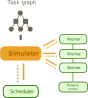
\includegraphics[scale=0.35]{estee/estee-architecture}
	\caption{\estee{} architecture}
	\label{fig:estee-architecture}
\end{figure}

\estee{} provides abstract interfaces for the task scheduler, the worker and the
network model (which simulates network communication and congestion). Users can thus easily provide
their own implementations of these interfaces, and in turn override both the behavior of the
scheduler and of the cluster and its network topology.

One of our goals for \estee{} was to make it very easy to write new scheduling
algorithms and make the scheduler approachable for other researchers that might want to experiment
with task schedulers. That was also one of the motivations why we decided to create
\estee{} in Python, which facilitates experimentation. Listing~\ref{lst:estee-example}
shows an example of a task graph simulation that demonstrates the simplicity of defining task graph
simulation using\estee{}. The output of the simulation is both the makespan (the duration it
took to execute the task graph) and also a detailed trace that can be used to visualize the
individual task-to-worker assignments and task execution time spans.

\begin{listing}
	\caption{Simple task graph simulation example using \estee{}}
	\label{lst:estee-example}
	\begin{minted}[fontsize=\small]{python}
# Create task graph containing 3 tasks
# (each task runs for 1s and requires 1 CPU)
#
#     t0
#     | (50MB output)
#    / \
#  t1   t2
tg = TaskGraph()
t0 = tg.new_task(duration=1, cpus=1, output_size=50)
t1 = tg.new_task(duration=1, cpus=1)
t1.add_input(t0)
t2 = tg.new_task(duration=1, cpus=1)
t2.add_input(t0)

# Create a task scheduler
scheduler = BlevelGtScheduler()

# Define cluster with 2 workers (1 CPU each)
workers = [Worker(cpus=1) for _ in range(2)]

# Define MaxMinFlow network model (100MB/s bandwidth)
netmodel = MaxMinFlowNetModel(bandwidth=100)

# Run simulation, returns the makespan in seconds
simulator = Simulator(tg, workers, scheduler, netmodel, trace=True)
makespan = simulator.run()
print(f"Task graph execution makespan = {makespan}s")
\end{minted}
\end{listing}

\section{Task scheduler benchmarks}
\label{sec:estee-benchmarks}
We have performed an extensive analysis of several task scheduling algorithms using
\estee{}.

%EXPAND: describe graph generator

Our analysis has shown that despite its simplicity, the foundational HLFET
algorithm~\cite{hlfet1974} produces high quality schedules in various scenarios and should
thus serve as a good baseline scheduler for task runtimes. We have also found out that even a
completely random scheduler can be competitive with other scheduling approaches for certain task
graphs and cluster configurations.

%During our attempts to implement various scheduling algorithms, we have also realized that the
%descriptions of many task scheduling algorithms in existing literature is incomplete. More
%specifically, seemingly inconsequential implementation details that are often missing from the
%algorithm's description can have a very large effect on the final performance of the scheduler,
%which makes it difficult to precisely reproduce and compare the performance of the existing
%algorithms.

%EXPAND: show Estee charts, describe the results in more detail

% List-Scheduling versus Cluster-Scheduling
% - simple schedulers are surprisingly competitive
